\documentclass[10pt,a4paper]{report}
\usepackage[utf8]{inputenc}
\usepackage[english]{babel}
\usepackage{amsmath}
\usepackage{amsfonts}
\usepackage{amssymb}
\usepackage{graphicx}
\usepackage[left=2cm,right=2cm,top=2cm,bottom=2cm]{geometry}
\usepackage{hyperref}
\author{Daniele Gilio}
\title{Sentiment Analysis on Imdb Database}
\begin{document}
\maketitle
\section{Introduction}
For this assignment we are going to perform sentiment analysis on film reviews from the popular Imdb site. In order to do that we were asked to build a Na\"{i}ve Bayesian Classifier able to assign a binary class (good or bad) given the word content of the review itself. The dataset is made of $25000$ training samples, $12500$ validation samples and $12500$ test samples.
\section{Data Preprocessing}
The first thing needed to make the Na\"{i}ve Bayesian Classifier work is some data processing. A crucial passage is the creation of a dictionary which we will use to build a Bag of Words representation of the reviews. To do that we scan all the training documents, clean the inputs by removing unwanted characters and record the frequency of appearance of each word, then we select the $n$-most frequent ones. The choice of $n$ is obviously going to affect the classifier performance. After the dictionary is built, we proceed to create the BoW representation of the documents which is basically a matrix in which columns represent the word in the dictionary and rows documents. The entries in the matrix are then the frequencies of occurrence of each word in each document. 
\section{Classification}
We used the pvml library to build our Na\"{i}ve Bayesian Classifier, which by means of Laplacian smoothing, ensures that we never encounter a zero probability. The Na\"{i}ve Bayesian Classifier has a very low computation time expense since it does not require SGD optimization. On the other hand this kind of classifier might not be the most versatile and makes a strong assumption on the dataset (the data items MUST be conditionally independent). Since in reality this is not always the case the Na\"{i}ve Bayesian Classifier might suffer performance-wise if compared with other classifiers. Its simplicity though makes it a very good starting point in tasks like sentiment analysis. Given these premises we also built an SVM classifier and a Logistic Regression one. For our baseline training we chose $n=1000$, the results we obtained can be seen in Table \ref{tab:baseline_training}.
\begin{table}[!ht]
\centering
\begin{tabular}{|l|c|c|c|}
\hline
 & \multicolumn{1}{l|}{Training Accuracy {[}\%{]}} & \multicolumn{1}{l|}{Validation Accuracy {[}\%{]}} & \multicolumn{1}{l|}{Test Accuracy {[}\%{]}} \\ \hline
Bayes  & 82.004 & 82.064 & 81.632 \\ \hline
SVM    & 87.432 & 86.528 & 86.192 \\ \hline
LogReg & 86.492 & 85.995 & 85.712 \\ \hline
\end{tabular}
\caption{Baseline Training Results}
\label{tab:baseline_training}
\end{table}
As we can see our concerns about the performance of the Na\"{i}ve Bayesian Classifier revealed to be true, even if the performance difference is of a couple of percentage points.
\section{Classification Variants}
In the assignment we were hinted to use more preprocessing techniques that may lead to performance improvements, which were Common Word Exclusion and Stemming\footnote{For this technique we used the Porter Stemming Algorithm provided with the dataset}. The first one, as the name implies, consists in discarding common word which do not carry much useful information. The second one can be regarded as a normalization technique, the words are basically cut to their roots, e.g. "running" becomes "run". The results of the application of these techniques are shown in Tables \ref{tab:ignore_common}, \ref{tab:stemming} and \ref{tab:stemming_ignore_common}.
\begin{table}[!ht]
\centering
\begin{tabular}{|l|c|c|c|}
\hline
 & \multicolumn{1}{l|}{Training Accuracy {[}\%{]}} & \multicolumn{1}{l|}{Validation Accuracy {[}\%{]}} & \multicolumn{1}{l|}{Test Accuracy {[}\%{]}} \\ \hline
Bayes  & 82.92  & 82.992  & 82.576 \\ \hline
SVM    & 86.98  & 85.351  & 85.536 \\ \hline
LogReg & 85.988 & 84.8639 & 84.894 \\ \hline
\end{tabular}
\caption{Ignore Common Words Results}
\label{tab:ignore_common}
\end{table} 

\begin{table}[!ht]
\centering
\begin{tabular}{|l|c|c|c|}
\hline
 & \multicolumn{1}{l|}{Training Accuracy {[}\%{]}} & \multicolumn{1}{l|}{Validation Accuracy {[}\%{]}} & \multicolumn{1}{l|}{Test Accuracy {[}\%{]}} \\ \hline
Bayes  & 82.32  & 81.94  & 81.624 \\ \hline
SVM    & 87.44  & 86.236 & 86.048 \\ \hline
LogReg & 86.632 & 85.688 & 85.784 \\ \hline
\end{tabular}
\caption{Stemming Results}
\label{tab:stemming}
\end{table} 

\begin{table}[!ht]
\centering
\begin{tabular}{|l|c|c|c|}
\hline
 & \multicolumn{1}{l|}{Training Accuracy {[}\%{]}} & \multicolumn{1}{l|}{Validation Accuracy {[}\%{]}} & \multicolumn{1}{l|}{Test Accuracy {[}\%{]}} \\ \hline
Bayes  & 82.54  & 82.296 & 81.888 \\ \hline
SVM    & 86.848 & 85.576 & 85.56  \\ \hline
LogReg & 86.144 & 85.264 & 85.168 \\ \hline
\end{tabular}
\caption{Stemming + Ignore Common Words Results}
\label{tab:stemming_ignore_common}
\end{table}
All the results above were produced while keeping every parameter constant. We can observe that the application of the described techniques improves the performance of all the models most of the times. From now on we will keep using both since it seems that that is the most balanced choice.
\section{Hyperparameters}
\subsection{Dictionary Size}
As we previously stated the dictionary size is a very important parameter because it carries the most information content given to the model. In order to verify that and to find the best size for our purposes we trained all the classifiers varying only the dictionary size. Figure \ref{fig:test_acc} shows the plot of Test Accuracy against dictionary size.
\begin{figure}[!ht]
\centering
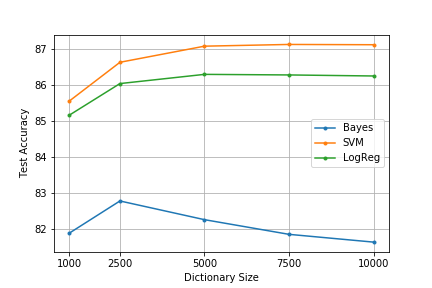
\includegraphics[width=0.4\linewidth]{test_acc.png}
\caption{Test Accuracies vs Dictionary Size}
\label{fig:test_acc}
\end{figure}
We can see a very clear peak at $n=2500$ for the Na\"{i}ve Bayesian Classifier, whereas the SVM and the LogReg increase until $n=5000$ and then remain constant. We can conclude that the optimal values are those ones both in terms of accuracy and computation time.
\subsection{Learning Rate, Steps and Regularization (SVM \& LogReg)}
After a couple of quick tests we determined that the optimal number of steps is $2000$ and the regularization values are $0.0001$ for the SVM and $0$ for the LogReg. We did not perform a proper grid search due to the long computation time required. The Learning Rate was a little bit more challenging: we started trying with a fixed one but the result were not satisfactory, they were on par or under the Na\"{i}ve Bayesian Classifier. After a little bit of online research we settled on an inverse scaling learning rate, basically the learning rate is initialized as $\gamma_0=1$ and updated according to:
\begin{equation}
\gamma(t)=\frac{\gamma_0}{\sqrt{t}}
\end{equation}
where $t$ is the number of steps.
\section{Results Analysis}
\section{Conclusions}
\end{document}